\section*{SCHEDULE 1 - PARTY DETAILS AND INITIAL SHAREHOLDINGS}

This Schedule is referenced in the Agreement dated 9 June 2025 between the parties.

\subsection*{Part A: The Company}
\begin{tabularx}{\textwidth}{@{} l X @{}}
\textbf{Name:} & The Augmented 4 Pty Ltd \\
\textbf{ACN:} & 686 749 575 \\
\textbf{Registered Office:} & Unit 4, 5 Norman Avenue, Dolls Point, \\
& New South Wales 2219, Australia \\
\textbf{Address for Notices:} & Unit 4, 5 Norman Avenue, Dolls Point, \\
& New South Wales 2219, Australia \\
& Attn: The Directors
\end{tabularx}

\vspace{1em}

\subsection*{Part B: The Shareholders}

\subsubsection*{Shareholder A}
\begin{tabularx}{\textwidth}{@{} l X @{}}
\textbf{Name:} & Domenico Rutigliano \\
\textbf{Position:} & Founder and Chief Technology Officer (CTO) \\
\textbf{Address for Notices:} & Unit 2, 5-7 Hercules Road, \\
& Brighton-le-Sands, NSW 2216, Australia \\
\textbf{Email:} & dom@ta4.ai \\
\textbf{Phone:} & +61 421 904 200 \\
\textbf{Initial Shareholding:} & 5,000,000 Ordinary Shares (Voting) \\
\textbf{Percentage of Total Authorized Shares:} & 42\% \\
\textbf{Voting Control:} & 50\% of voting shares
\end{tabularx}

\vspace{1em}

\subsubsection*{Shareholder B}
\begin{tabularx}{\textwidth}{@{} l X @{}}
\textbf{Name:} & Michael Scheelhardt \\
\textbf{Position:} & Chief Revenue Officer (CRO) \\
\textbf{Address for Notices:} & Unit 4, 5 Norman Avenue, Dolls Point, \\
& NSW 2219, Australia \\
\textbf{Email:} & michael@ta4.ai \\
\textbf{Phone:} & +61 404 971 242 \\
\textbf{Initial Shareholding:} & 5,000,000 Ordinary Shares (Voting) \\
\textbf{Percentage of Total Authorized Shares:} & 42\% \\
\textbf{Voting Control:} & 50\% of voting shares
\end{tabularx}

\vspace{1em}

\subsection*{Part C: Authorized Capital Structure}
\begin{tabularx}{\textwidth}{@{} l X @{}}
\textbf{Total Authorized Shares:} & 11,904,762 \
\textbf{Total Issued Shares:} & 10,000,000 \
\textbf{Reserved Share Pool:} & 1,904,762 (16\%)
\end{tabularx}

\vspace{1em}

\subsubsection*{Share Class Breakdown}
\begin{tabularx}{\textwidth}{@{} l l l l @{}}
\textbf{Share Class} & \textbf{Authorized} & \textbf{Issued} & \textbf{Percentage} \\
\hline
Ordinary Shares (Voting) & 10,000,000 & 10,000,000 & 84\% \\
Preference Shares (Non-Voting) & 1,190,476 & 0 & 10\% \\
Employee Ordinary Shares (Non-Voting) & 714,286 & 0 & 6\% \\
\hline
\textbf{Total} & \textbf{11,904,762} & \textbf{10,000,000} & \textbf{100\%} \\
\end{tabularx}

\vspace{1em}

\subsection*{Part D: Share Class Definitions and Rights}

\subsubsection*{Class 1: Ordinary Shares (Voting)}
\begin{tabularx}{\textwidth}{@{} l X @{}}
\textbf{Holders:} & Founders (Domenico Rutigliano and Michael Scheelhardt) \\
\textbf{Voting Rights:} & 1 vote per share on all matters \\
\textbf{Dividend Rights:} & Pro-rata participation after preference dividends \\
\textbf{Liquidation Rights:} & Pro-rata participation after preference liquidation \\
\textbf{Transfer Rights:} & Subject to pre-emptive rights and Board approval \\
\textbf{Conversion Rights:} & None (base class) \\
\textbf{Current Allocation:} & 10,000,000 shares (84\% of total authorized)
\end{tabularx}

\vspace{1em}

\subsubsection*{Class 2: Preference Shares (Non-Voting)}
\begin{tabularx}{\textwidth}{@{} l X @{}}
\textbf{Holders:} & Strategic investors and institutional investors \\
\textbf{Voting Rights:} & None, except on matters specifically affecting this class \\
\textbf{Dividend Rights:} & Cumulative 8\% preference dividend (if declared) \\
\textbf{Liquidation Preference:} & 1x non-participating liquidation preference \\
\textbf{Anti-Dilution:} & Weighted average broad-based anti-dilution protection \\
\textbf{Information Rights:} & Monthly management accounts, annual audited accounts \\
\textbf{Board Rights:} & Right to appoint one non-voting board observer \\
\textbf{Transfer Rights:} & Tag-along and drag-along participation rights \\
\textbf{Conversion Rights:} & Optional conversion to Ordinary Shares (Voting) \\
\textbf{Reserved Allocation:} & 1,190,476 shares (10\% of total authorized)
\end{tabularx}

\vspace{1em}

\subsubsection*{Class 3: Employee Ordinary Shares (Non-Voting)}
\begin{tabularx}{\textwidth}{@{} l X @{}}
\textbf{Holders:} & Employees, advisors, consultants, and service providers \\
\textbf{Voting Rights:} & None \\
\textbf{Dividend Rights:} & Pro-rata participation after preference dividends \\
\textbf{Liquidation Rights:} & Pro-rata participation after preference liquidation \\
\textbf{Vesting:} & Subject to employment-based vesting schedules \\
\textbf{Transfer Rights:} & Restricted; Company right of first refusal \\
\textbf{Tax Benefits:} & Eligible for Australian ESS tax concessions \\
\textbf{Conversion Rights:} & None \\
\textbf{Reserved Allocation:} & 714,286 shares (6\% of total authorized)
\end{tabularx}

\vspace{1em}

\subsection*{Part E: Voting Control and Governance}
\begin{tabularx}{\textwidth}{@{} l X @{}}
\textbf{Total Voting Shares:} & 10,000,000 Ordinary Shares (Voting) \\
\textbf{Founder Voting Control:} & 100\% of voting shares (50\% each) \\
\textbf{Board Control:} & Founders maintain majority board control \\
\textbf{Reserved Matters:} & Require unanimous founder approval \\
\textbf{Investor Protection:} & Through preference rights, not voting control \\
\textbf{Employee Participation:} & Economic rights only, no governance rights
\end{tabularx}

\section*{Share Distribution Structure and Rationale}

\subsection*{Share Distribution Overview}

\begin{tabularx}{\textwidth}{@{} l r r l l @{}}
\textbf{Shareholder Category} & \textbf{Shares} & \textbf{Percentage} & \textbf{Share Class} & \textbf{Voting Rights} \\
\hline
Domenico Rutigliano & 5,000,000 & 42\% & Ordinary (Voting) & Full voting control \\
Michael Scheelhardt & 5,000,000 & 42\% & Ordinary (Voting) & Full voting control \\
Future Investors & 1,190,476 & 10\% & Preference (Non-Voting) & Economic rights only \\
Future Employees & 714,286 & 6\% & Ordinary (Non-Voting) & Economic rights only \\
\hline
\textbf{TOTAL} & \textbf{11,904,762} & \textbf{100\%} & & \\
\end{tabularx}

\subsection*{Structural Design Rationale}

\subsubsection*{Even Founder Distribution (42\% each)}
\begin{itemize}
    \item \textbf{Equal Partnership:} Both founders have identical stakes, preventing control disputes
    \item \textbf{Shared Decision Making:} All major decisions require both founders' agreement
    \item \textbf{Fair Compensation:} Equal reward for equal commitment and risk
    \item \textbf{Clean Numbers:} 5,000,000 shares each provides easy calculation and understanding
\end{itemize}

\subsubsection*{Reserved Pool Percentages (10\% + 6\%)}
\begin{itemize}
    \item \textbf{Mathematical Precision:} 10\% equals exactly 1,190,476 shares; 6\% equals exactly 714,286 shares
    \item \textbf{Market Standards:} 10\% investor pool aligns with typical early-stage allocation; 6\% employee pool appropriate for small team startup
    \item \textbf{Founder Control Preservation:} Founders maintain 84\% combined ownership and 100\% voting control
    \item \textbf{Equal Dilution:} Pools dilute founders proportionally, maintaining their relative equality
\end{itemize}

\subsection*{Strategic Benefits}

\subsubsection*{Control Structure}
\begin{itemize}
    \item \textbf{Founders:} 100\% voting control through Ordinary Voting shares
    \item \textbf{Investors:} Economic participation without governance interference
    \item \textbf{Employees:} Economic incentives without diluting founder control
\end{itemize}

\subsubsection*{Growth Flexibility}
\begin{itemize}
    \item \textbf{Investor Pool:} Ready for funding rounds without complex restructuring
    \item \textbf{Employee Pool:} Attracts talent with equity participation
    \item \textbf{Scalable:} Structure works from startup to large company
\end{itemize}

\subsubsection*{Mathematical Logic}
\begin{itemize}
    \item \textbf{Why not 50/50 founders:} 50/50 allocation leaves no room for growth pools
    \item \textbf{42/42/10/6 structure:} Maintains founder equality while enabling expansion
    \item \textbf{Pool sizing rationale:} 10\% investors provides Series A readiness; 6\% employees sufficient for 5-10 key hires
    \item \textbf{Total pool allocation:} 16\% total pools provides meaningful but not excessive dilution
\end{itemize}

This structure balances founder equality, growth capacity, and control preservation in a mathematically clean and legally sound framework.

\subsection*{Share Structure Diagram}

\begin{center}
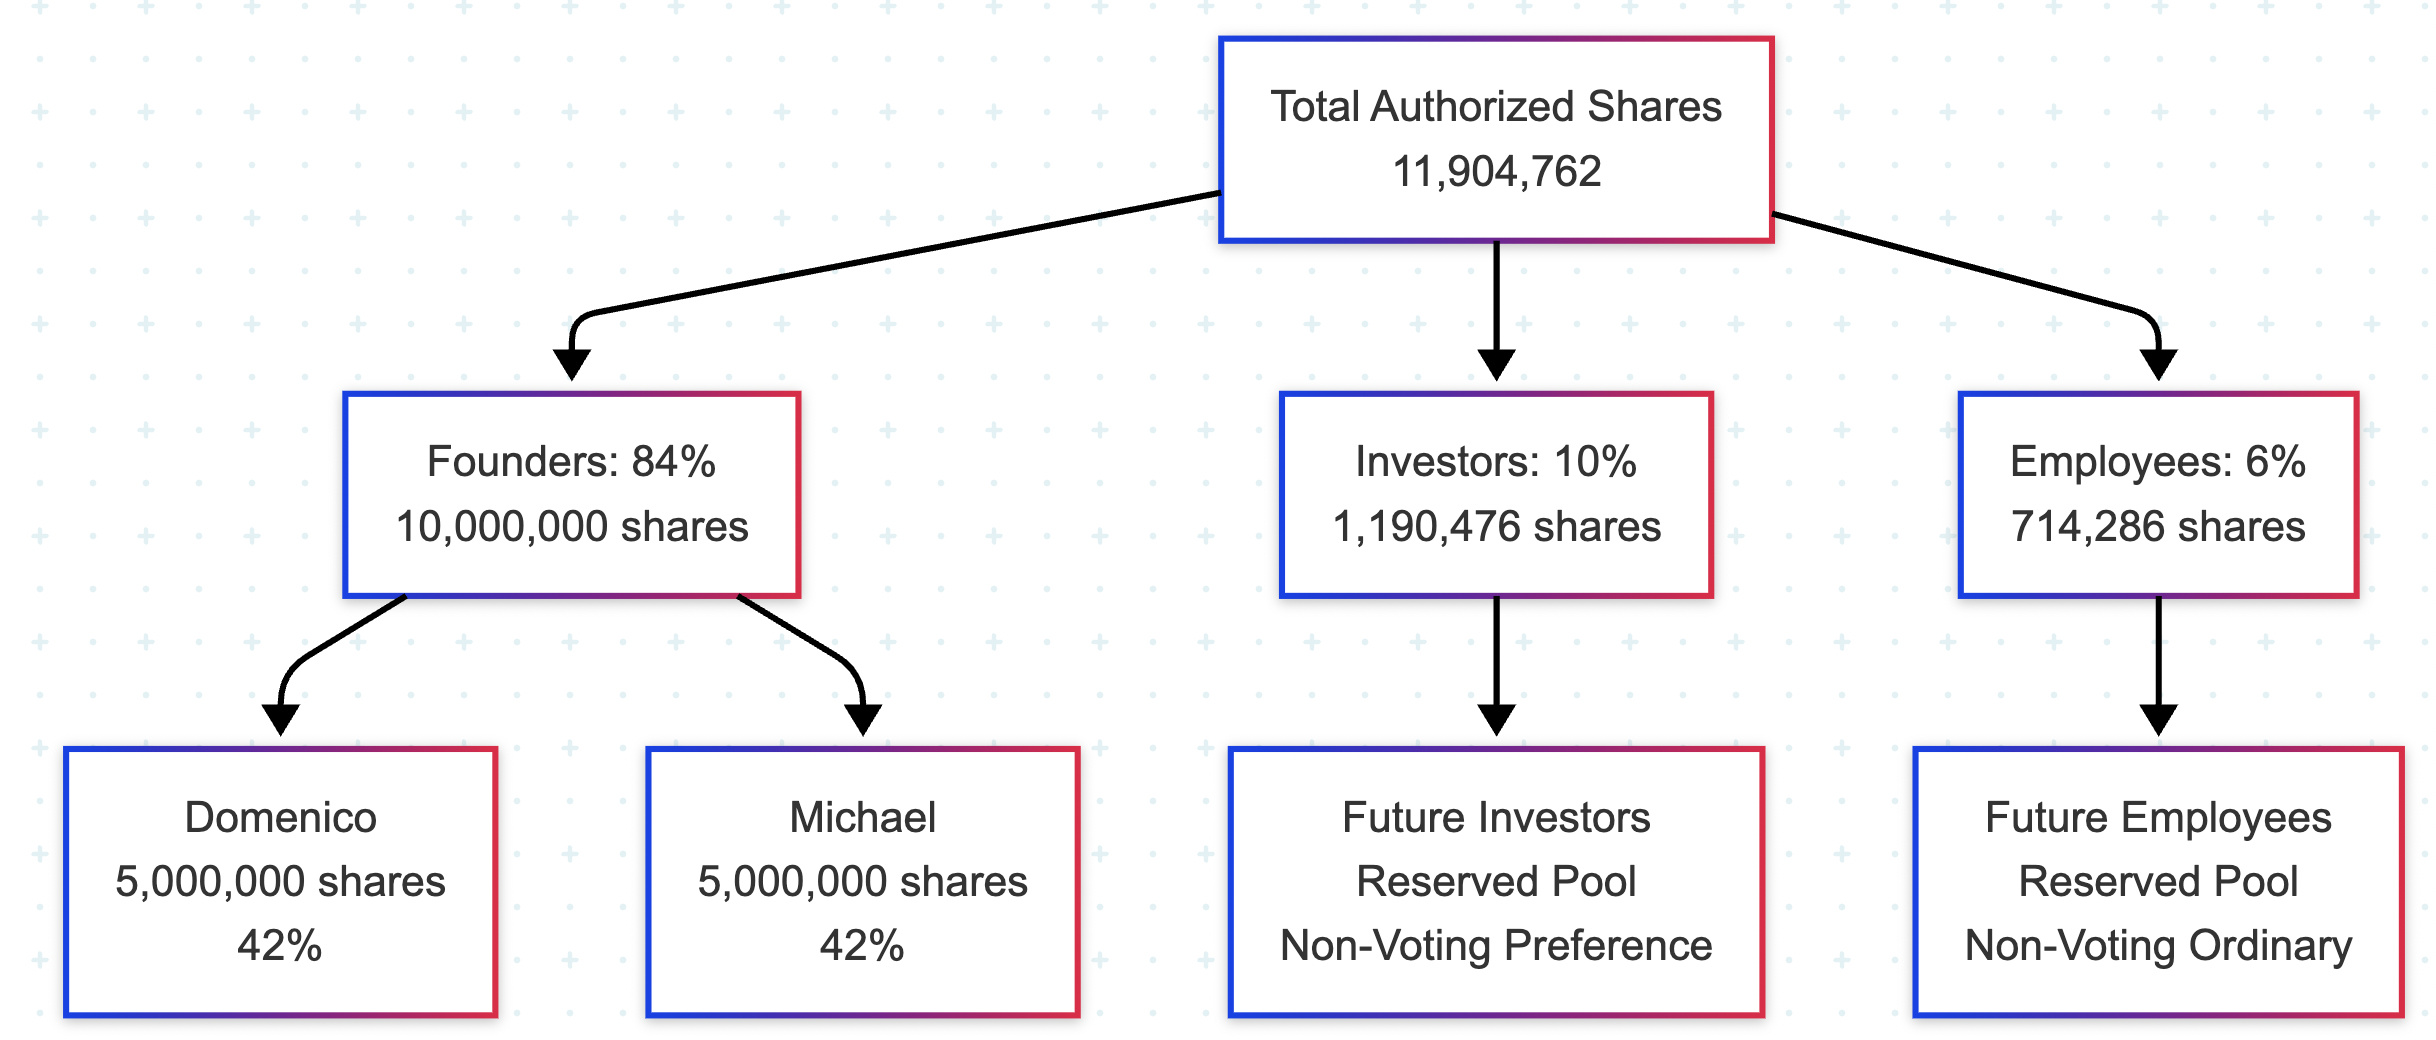
\includegraphics[width=0.9\textwidth]{/Users/domrutili/PROJECTS/Augmented-4-ShareHolder-Agreement/images/shares.png}
\end{center}

\textbf{Diagram Description:} The above diagram illustrates the hierarchical distribution of The Augmented 4 Pty Ltd's authorized share capital. At the top level, the total authorized shares of 11,904,762 are divided into three main categories: Founders (84\% - 10,000,000 shares), Investors (10\% - 1,190,476 shares), and Employees (6\% - 714,286 shares). The Founders category is further subdivided equally between Domenico and Michael, each holding 5,000,000 shares representing 42\% of the total. The Investor and Employee categories represent reserved pools for future allocation, with investors receiving Non-Voting Preference shares and employees receiving Non-Voting Ordinary shares. This visual representation demonstrates the balanced approach to equity distribution while maintaining founder control through voting rights concentration.

\textit{Note: This structure ensures founder control while providing appropriate investor protections and employee economic participation. All share issuances from reserved pools require unanimous Board approval and compliance with this Agreement.} 